\documentclass[11pt]{article}
\usepackage[margin=1in]{geometry}
\usepackage[T1]{fontenc}
\usepackage{lmodern}
\usepackage{microtype}
\usepackage{graphicx}
\usepackage{booktabs}
\usepackage{amsmath}
\usepackage{caption}
\usepackage{float}
\usepackage[hidelinks]{hyperref}

\graphicspath{{figures/}}
\captionsetup{font=small,labelfont=bf}

% ---- fill these in ---------------------------------------------------------
\newcommand{\authorone}{Prad R.}            % TODO: full name
\newcommand{\authortwo}{[Teammate name]}    % TODO: teammate's name
% ----------------------------------------------------------------------------

% final-submission numbers (from results/best/latest/summary.json)
\newcommand{\BestDone}{0.052}
\newcommand{\BestDtwo}{0.219}
\newcommand{\BestDthree}{0.441}
\newcommand{\JointsOne}{4--14}
\newcommand{\JointsTwo}{4--15}
\newcommand{\JointsThree}{2--19}

\title{2.156 Challenge Problem 1: Linkage Synthesis\\[2pt]
\large Screening, gradient refinement and growth of planar linkages}
\author{\authorone \and \authortwo}
\date{October 2026}

\begin{document}
\maketitle

\begin{abstract}
\noindent We design planar linkages whose traced curve matches three kangaroo
outlines while using as little link material as possible. Our pipeline is a mass
random screen of about 21 million mechanisms, gradient refinement of the best
of them, a growth stage that adds one joint at a time, a second, much wider
refinement, and a second round of growth. The final submission scores \textbf{3.69} with the course
scorer (hypervolumes 5.87, 8.52 and 24.60), up from 0.045 for the advanced
starter notebook. Most of the score comes from the screen and the first
refinement; after that, moving joints stopped helping and only changes to the
link layout still lowered the distance. The tail of Kangaroo~3 is the main
feature we do not capture.
\end{abstract}

\section{Problem}

A mechanism is a set of joints with initial positions, rigid links between
them, a set of grounded joints, one motor link, and one traced joint. Turning
the motor through a full revolution makes the traced joint draw a closed curve.
For each of three target curves we submit up to 1000 mechanisms of at most 20
joints, and each mechanism is judged on two objectives, both minimized:
\begin{itemize}
\item \textbf{Distance}: the mismatch between the traced curve and the target
after the best rotation and starting point. Scale is \emph{not} normalized, so
the curve has to be the right size as well as the right shape.
\item \textbf{Material}: the total length of all links.
\end{itemize}
A design counts only if it is strictly under both limits in
Table~\ref{tab:problems}. The score for a target is the hypervolume its designs
dominate relative to those limits, divided by a normalizer; the overall score is
the mean over the three targets.

\begin{table}[H]
\centering
\begin{tabular}{llccc}
\toprule
Problem & Target & Distance limit & Material limit & Normalizer \\
\midrule
1 & Kangaroo 1 (round body) & 0.75 & 10 & 2.0 \\
2 & Kangaroo 2 (no ears or tail) & 1.2 & 10 & 1.5 \\
3 & Kangaroo 3 (full outline) & 1.75 & 20 & 10.0 \\
\bottomrule
\end{tabular}
\caption{The three problems. The limits are both the validity cutoff and the
hypervolume reference point.}
\label{tab:problems}
\end{table}

Two properties of this setup shaped everything we did. First, scaling all joint
positions by a factor scales the traced curve and the material together, so
every mechanism has a free one-variable trade-off between the two objectives.
Second, the hypervolume a design adds is its distance gain times the material
headroom above it, so an accuracy gain on a cheap design is worth more than the
same gain on a heavy one.

\section{Approach}

Table~\ref{tab:stages} lists the stages in the order they ran and the official
score after each. All scores in this report come from the course function
\texttt{evaluate\_submission}.

\begin{table}[H]
\centering
\begin{tabular}{lp{8.3cm}c}
\toprule
Stage & What it does & Score after \\
\midrule
Starter notebook & Seeded NSGA-II, then gradient descent (Kangaroo 2 only) & 0.045 \\
1. Screening & Random mechanisms, pruned and resized, no optimization & 2.78 \\
2. Refinement & Adam on joint positions, four material weights per design & 3.43 \\
3. Growth & Add one traced joint with two links, refine, select; 20 generations & 3.50 \\
4. Wide refinement & About 4000 starts per target, successive halving & 3.67 \\
5. Growth, round two & Growth again from the wide results, inside the limits & 3.69 \\
\bottomrule
\end{tabular}
\caption{Pipeline stages and the overall score after each.}
\label{tab:stages}
\end{table}

\subsection{Stage 1: mass random screening}

We started by exploring instead of optimizing. The starter's genetic algorithm
found no feasible design from a random start and reached a score of only 0.045
when seeded, which suggested that the hard part was finding link layouts worth
optimizing at all. Random sampling also parallelizes trivially across cluster
workers, which a single evolving population does not.

Each worker repeatedly samples random mechanisms with 10 to 20 joints, built so
that every joint hangs off two earlier ones, with several random joint layouts
per link structure. All of them are solved in one batched call. We then treat
\emph{every} moving joint as a possible traced joint and prune its mechanism to
the joints that actually drive it, which removes links that only add material.
After pruning, the candidates have 4 to 9 joints.

Scoring every candidate with the official metric would be too slow, so the
candidates are first ranked by a cheap shape comparison (a Fourier-domain
least-squares alignment over all starting points, both directions, rotation and
scale). The best 40 per target in each batch are then scored with the official
metric at nine sizes around the best-fit scale, which turns each candidate into
several points along its own distance and material trade-off.

Four workers ran for about four hours each. In total they sampled 20.9 million
mechanisms, screened 91.8 million candidate curves, and made 22 million
official evaluations. With no optimization at all this gave a score of 2.78
(Figure~\ref{fig:screenfronts}). The gains flattened early: the score was
already 2.61 after the first worker-hour.

\begin{figure}[H]
\centering
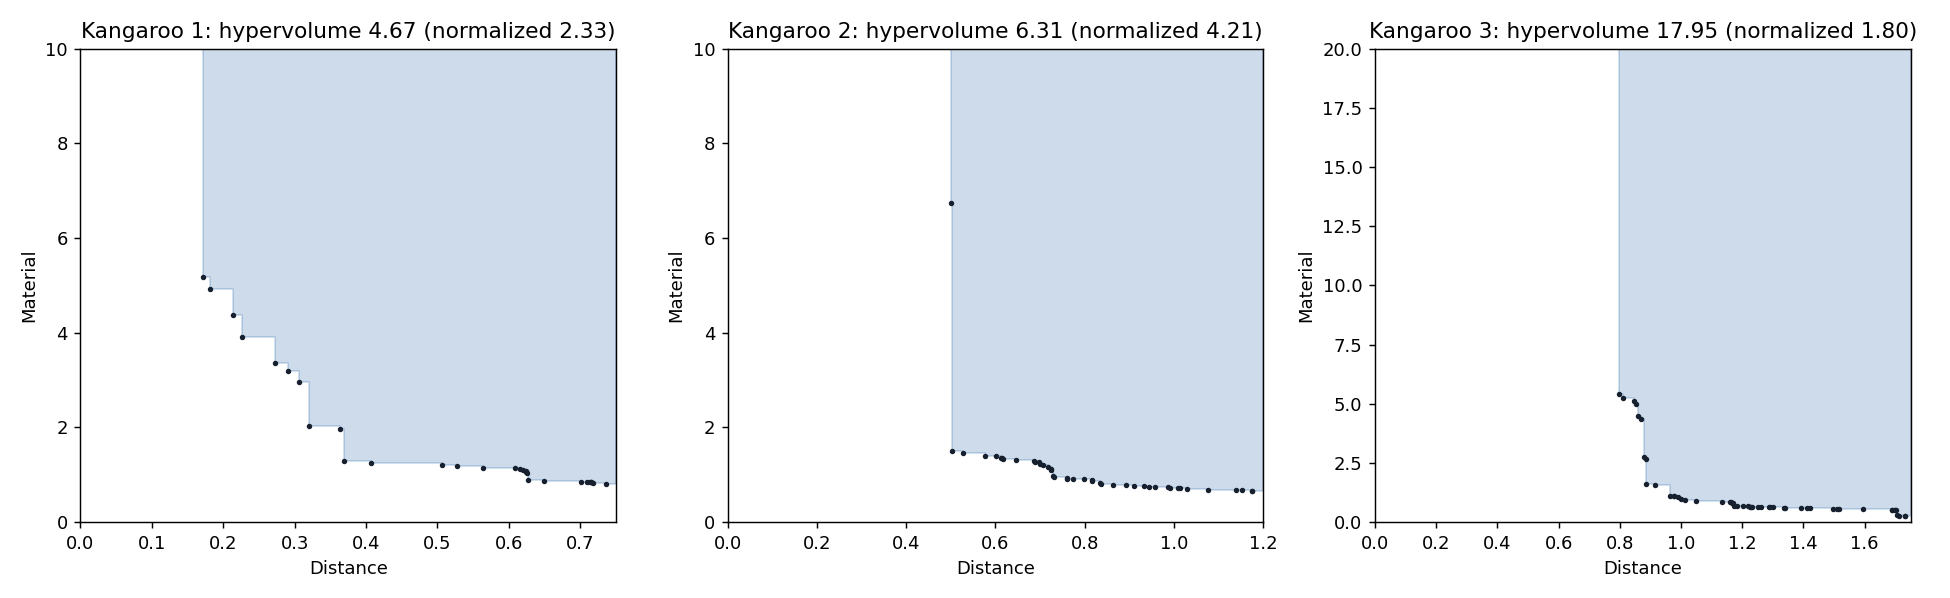
\includegraphics[width=\linewidth]{screen_fronts.png}
\caption{Pareto fronts after screening alone (score 2.78). Shaded area is the
hypervolume. Best distances are 0.17, 0.50 and 0.80.}
\label{fig:screenfronts}
\end{figure}

\subsection{Stage 2: gradient refinement}

For each target we took the most accurate screened designs, a fixed number per
joint count so that larger mechanisms were represented (136 designs per
target), and ran Adam on the joint positions for 1500 steps. Each design was
refined four times, minimizing
\[
  \text{distance} + w \cdot \text{material}, \qquad w \in \{0,\ 0.03,\ 0.1,\ 0.3\},
\]
so that one starting design spreads into several points along the front. Every
intermediate step that fell inside the limits was offered to the Pareto front,
not only the final one.

This raised the score from 2.78 to 3.43 and cut the best distances to 0.067,
0.30 and 0.48 (Figure~\ref{fig:progress}, blue). At this point the most accurate
Kangaroo~3 design followed both ears, but the tail and feet were still missed,
as were the snout and feet corners of Kangaroo~2.

\begin{figure}[H]
\centering
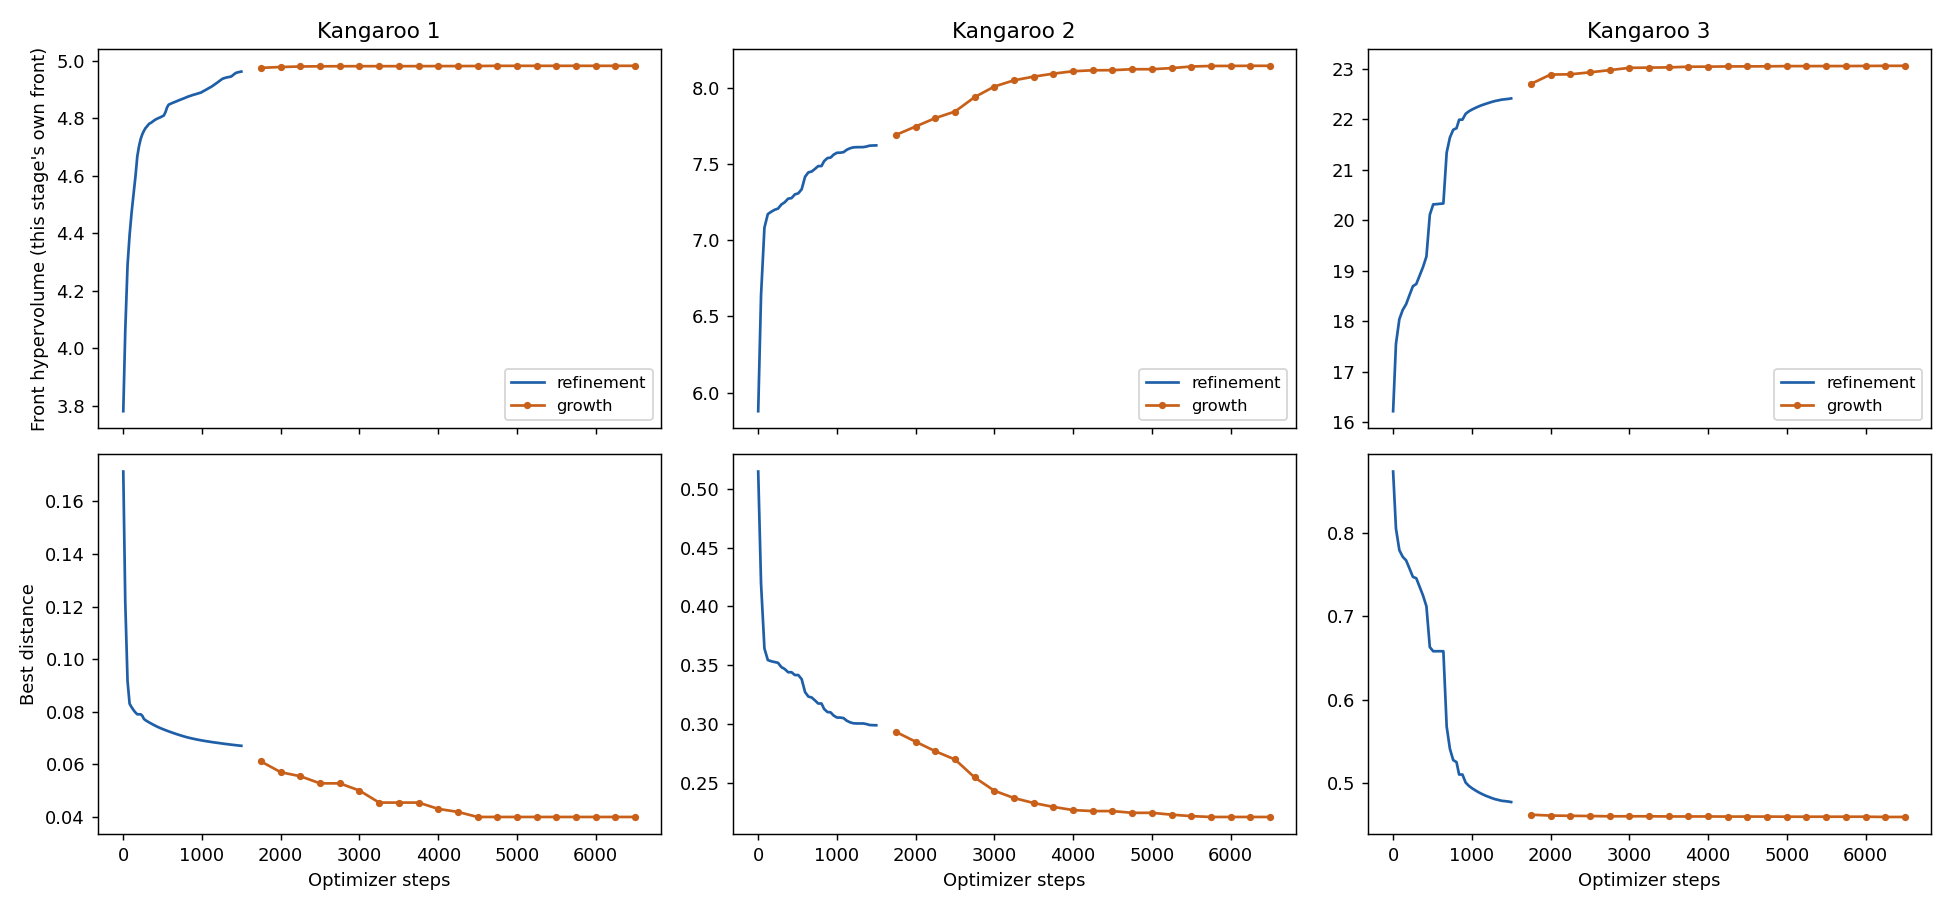
\includegraphics[width=\linewidth]{progress.png}
\caption{Hypervolume (top) and best distance (bottom) during refinement (blue)
and growth round one (orange, one marker per generation). Each curve is that
stage's own front, not the merged submission. In round one, growth selected
parents on distance alone, so the Kangaroo~1 curve ends at a 20-joint design
with distance 0.040 that is over the material limit and does not count; the
best valid Kangaroo~1 distance after this stage was 0.054.}
\label{fig:progress}
\end{figure}

\subsection{Stage 3: growth}

Refinement only moves joints; it cannot change which joints are connected. To
capture finer features we let designs grow. Each generation, every parent gets
96 children, each made by attaching \emph{one new traced joint with two links}
to the parent in one of three ways:
\begin{itemize}
\item to the old traced joint and one of its parents, which puts the new point
on the same rigid body, close to the old one, so the child starts out tracing
almost the same curve;
\item to any two existing joints;
\item to one moving joint and a new ground joint.
\end{itemize}
Children are pruned, resized to the target and scored. The best 512 are refined
for 250 Adam steps, and the next parents are the most accurate designs in each
joint-count bin, so small and large designs both survive.

Twenty generations raised the score to 3.50 and lowered the best distances to
0.054, 0.22 and 0.46. The largest effect was on Kangaroo~2 (0.30 to 0.22). The
last generation found no improving child on any target.

One flaw surfaced here: parents were chosen on distance alone, so some drifted
over the material limit and their gains did not count. We changed the selection
to keep parents inside the limits before the second round.

\subsection{Stage 4: wide refinement}

The first refinement had started from only 136 designs per target, and its best
results came from a few that happened to sit in good basins. It also contained
no four-joint designs, although those hold the low-material end of every front.
The wide round therefore restarts refinement from about 4000 candidates per
target: all screening seeds and fronts, the results of stages 2 and 3, and the
other two targets' best designs (the three outlines are versions of one shape).
No new random mechanisms were sampled. Steps are spent by successive halving: a
short run for all 4096, a longer one for the best 1024 (chosen per joint
count), and a long run at several material weights for the best 192 plus 64
cheap designs.

This raised the score from 3.50 to 3.67. Notably, it did \emph{not} improve the
best distance on any target. The whole gain came from cheaper designs at the
same accuracy, which is where hypervolume is most valuable.

\subsection{Stage 5: growth, round two}

Growth was run again from the wide results, with parents restricted to the
material limits. It made the last improvements on all three problems and brought
the score to 3.69. Every design set in the final file comes from this stage.

\section{Where the remaining error is}

Since the best distances had stopped moving, we measured the error point by
point along each target, aligning designs exactly as the scorer does
(Figure~\ref{fig:error3}).

\begin{itemize}
\item \textbf{Kangaroo 1} is matched closely everywhere.
\item \textbf{Kangaroo 2} has no single problem area. Its most accurate design
has several similar peaks, at the snout tip, the feet and the lower-right
corner. Cheap six-joint designs miss the concavity between snout and feet.
\item \textbf{Kangaroo 3} loses most on the tail, between 55 and 65\% of the
perimeter. For the most accurate design the worst fifth of the perimeter
carries 48\% of the distance. The ears are captured.
\end{itemize}

\begin{figure}[H]
\centering
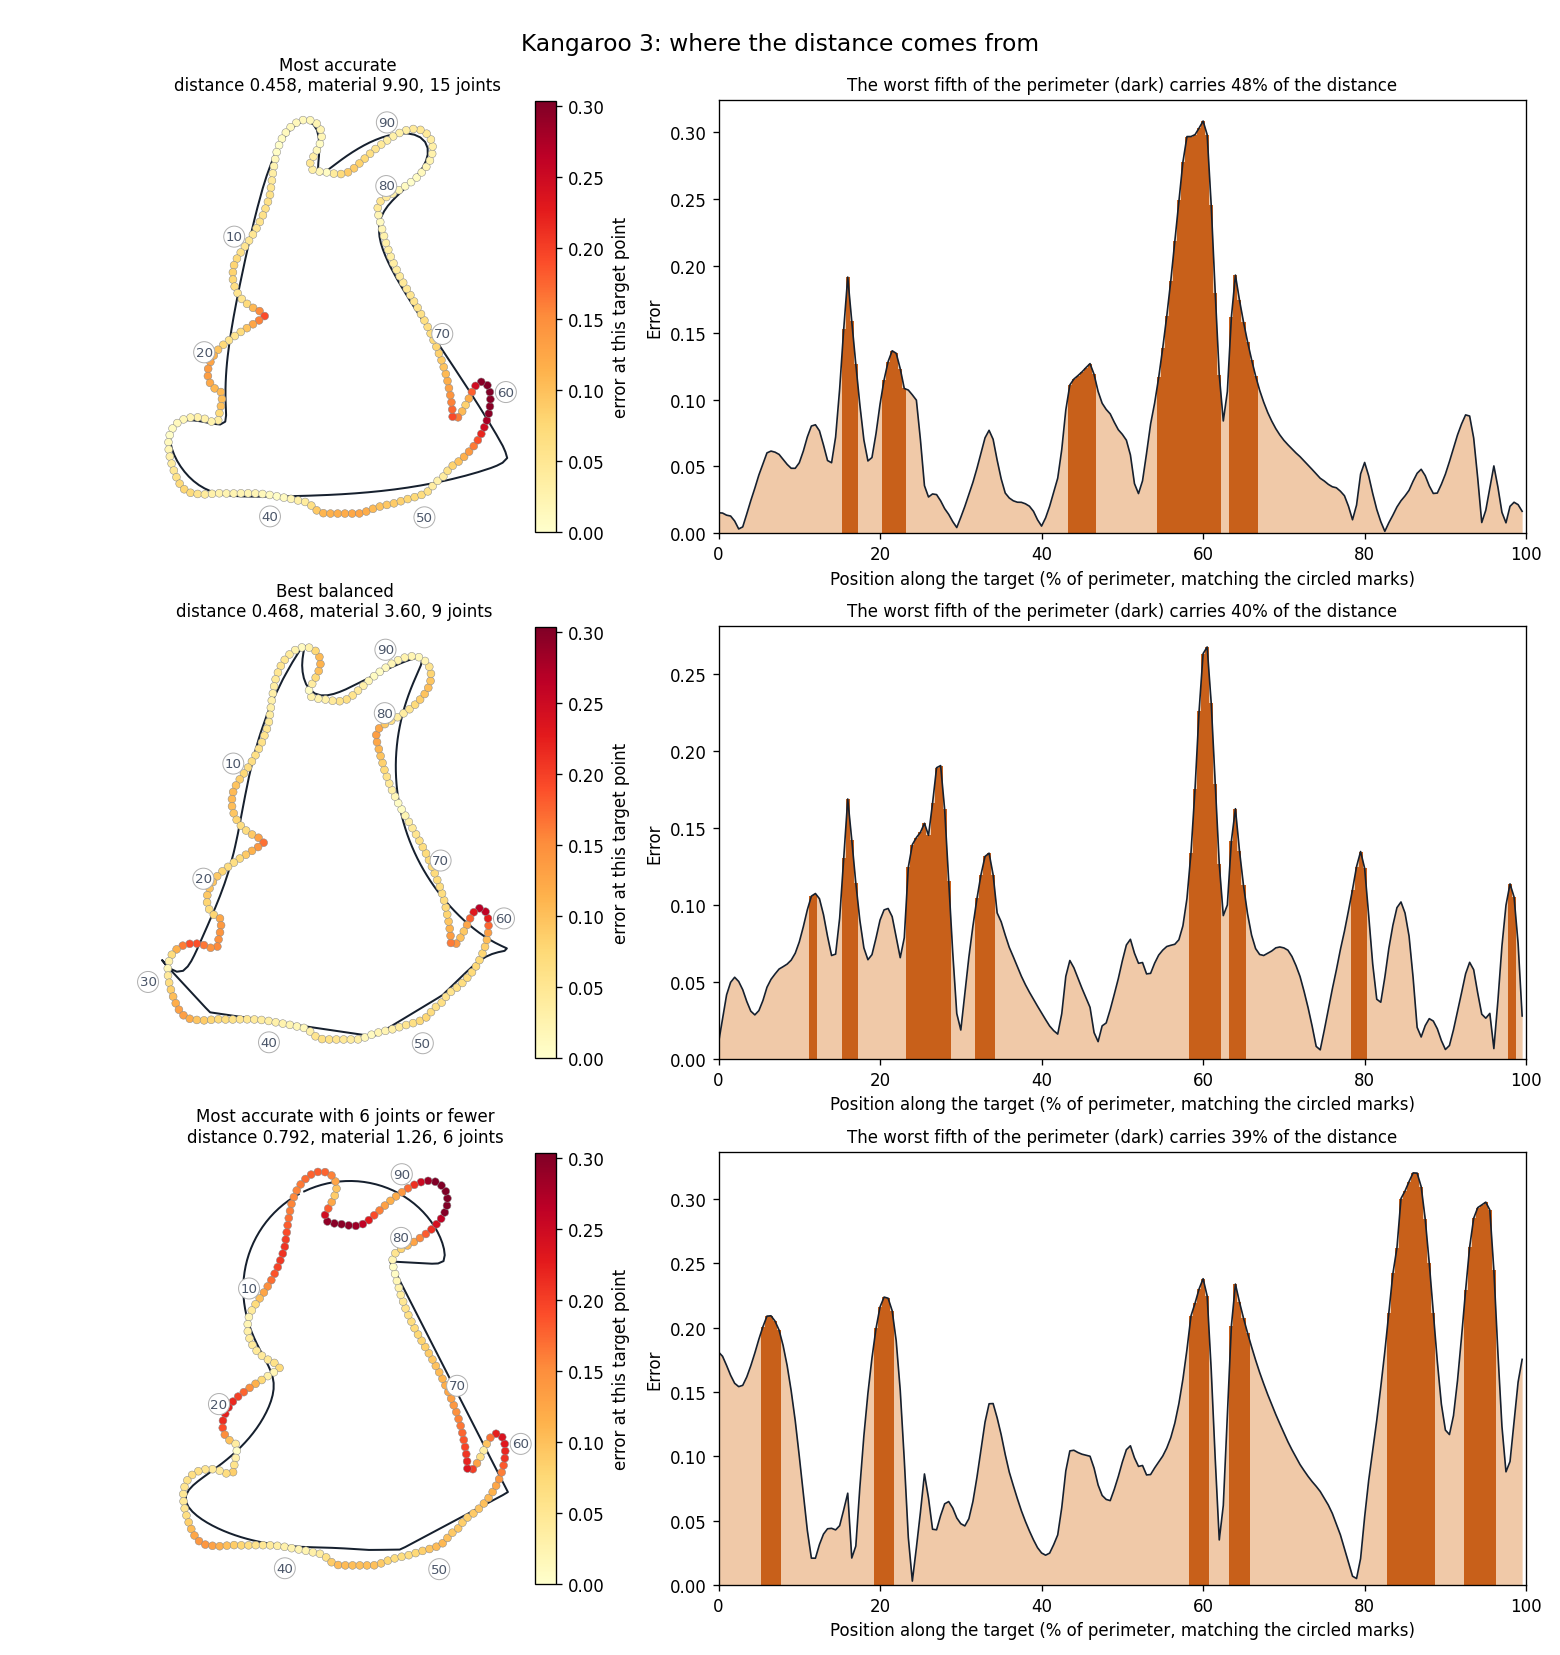
\includegraphics[width=0.86\linewidth]{error_3.png}
\caption{Kangaroo 3: error at each target point (left) and along the perimeter
(right) for three designs, as of the evening of October 5. The tail, near
60\% of the perimeter, dominates the most accurate design's distance.}
\label{fig:error3}
\end{figure}

The metric compares points at matching positions along the perimeter, so a
curve that reaches part of the way into a narrow feature such as the tail earns
little for it, and the optimizer has no easy path toward tracing it.

\subsection{Ideas that did not help}

We tested three ways of lowering distance without changing the link layout.
All were negative.

\begin{table}[H]
\centering
\begin{tabular}{p{3.2cm}p{7.2cm}p{4.0cm}}
\toprule
Idea & Test & Hypervolume change (K1 / K2 / K3) \\
\midrule
Assembly-branch flips & Mirror a moving joint across the line through its two
parents, keeping every link length, then refine. About 7000 flips. &
$+0.012$ / $+0.001$ / $+0.001$ \\
More forgiving losses & Refine first on a two-way nearest-point distance, or on
a blurred target sharpened in steps, then finish on the official distance.
Compared with a control on the same parents. &
Control matched or beat both on every target \\
Strictly improving polish & Accept only steps that improve one objective
without worsening the other. &
$+0.0007$ / $+0.0005$ / $+0.0012$ \\
\bottomrule
\end{tabular}
\caption{Experiments on joint positions only.}
\label{tab:negative}
\end{table}

The forgiving-loss test was our attempt to act on the tail diagnosis: if the
official distance gives little credit for a partly formed tail, a gentler loss
might lead the optimizer there. It did not. For Kangaroo~3 the control reached
a hypervolume of 24.36 against 24.27 and 24.19 for the two variants. A side
finding was that restarting Adam on converged designs usually left them worse
than they began, so the best point along the way has to be kept.

Together with the wide refinement, these results say the front designs sit at
true minima for their link layouts. Only structural change, the growth stage,
still lowered distance.

\section{Final results}

\begin{table}[H]
\centering\small
\begin{tabular}{lcccccc}
\toprule
Target & Designs & Hypervolume & Normalized & Best distance & Least material & Joints \\
\midrule
Kangaroo 1 & 1000 & 5.865 & 2.933 & \BestDone & 0.81 & \JointsOne \\
Kangaroo 2 & 1000 & 8.521 & 5.681 & \BestDtwo & 0.65 & \JointsTwo \\
Kangaroo 3 & 1000 & 24.604 & 2.460 & \BestDthree & 0.27 & \JointsThree \\
\midrule
Overall score & & & \textbf{3.691} & & & \\
\bottomrule
\end{tabular}
\caption{The final submission. The score was reproduced exactly (3.691214) by
scoring the file from a clean copy of the course repository in a fresh process.}
\label{tab:final}
\end{table}

\begin{figure}[H]
\centering
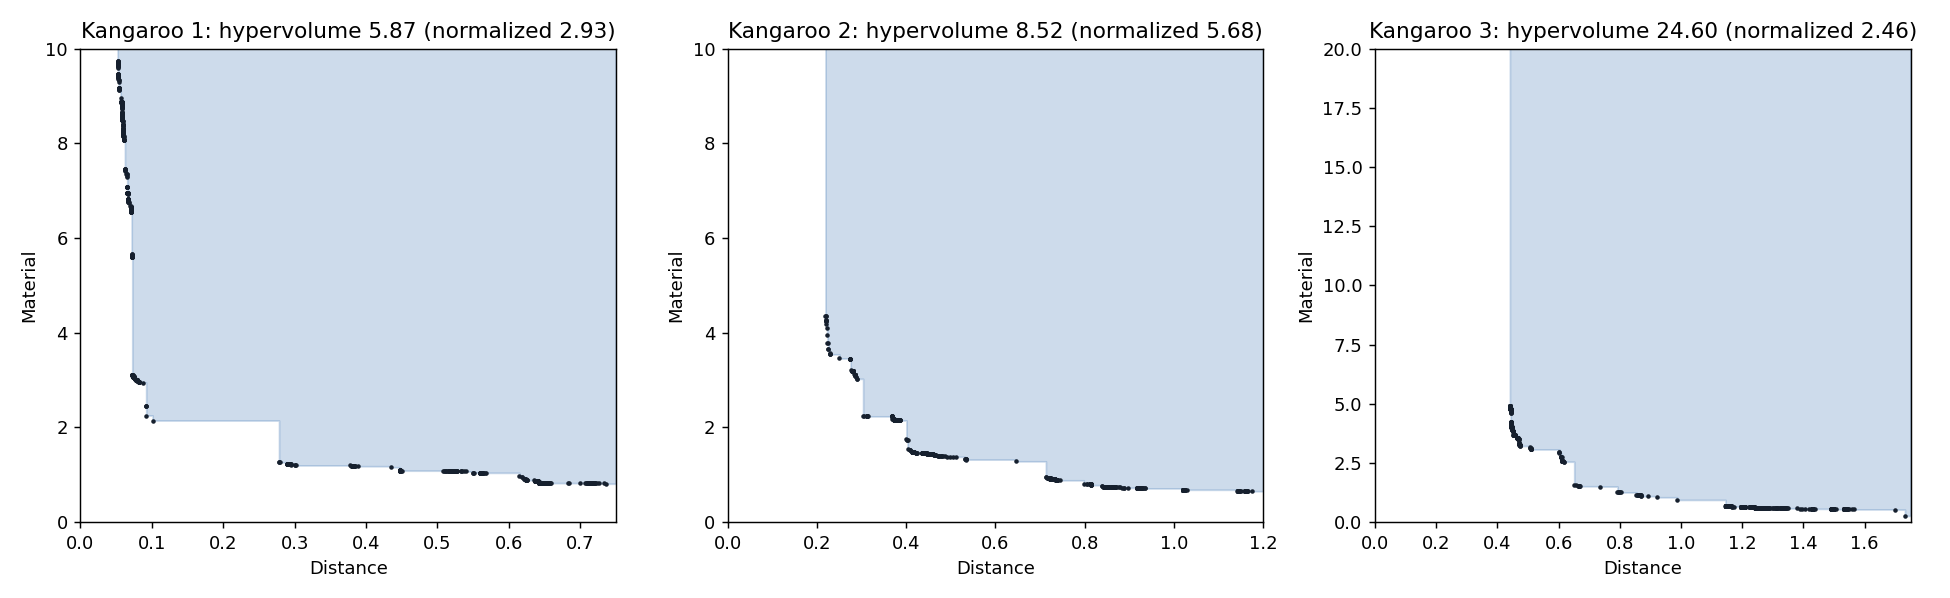
\includegraphics[width=\linewidth]{fronts.png}
\caption{Final Pareto fronts inside their limit boxes.}
\label{fig:fronts}
\end{figure}

Figures~\ref{fig:best1} to \ref{fig:best3} show, for each target, the most
accurate design, the best-balanced design (the one that alone dominates the
largest area) and the lightest design.

\begin{figure}[H]
\centering
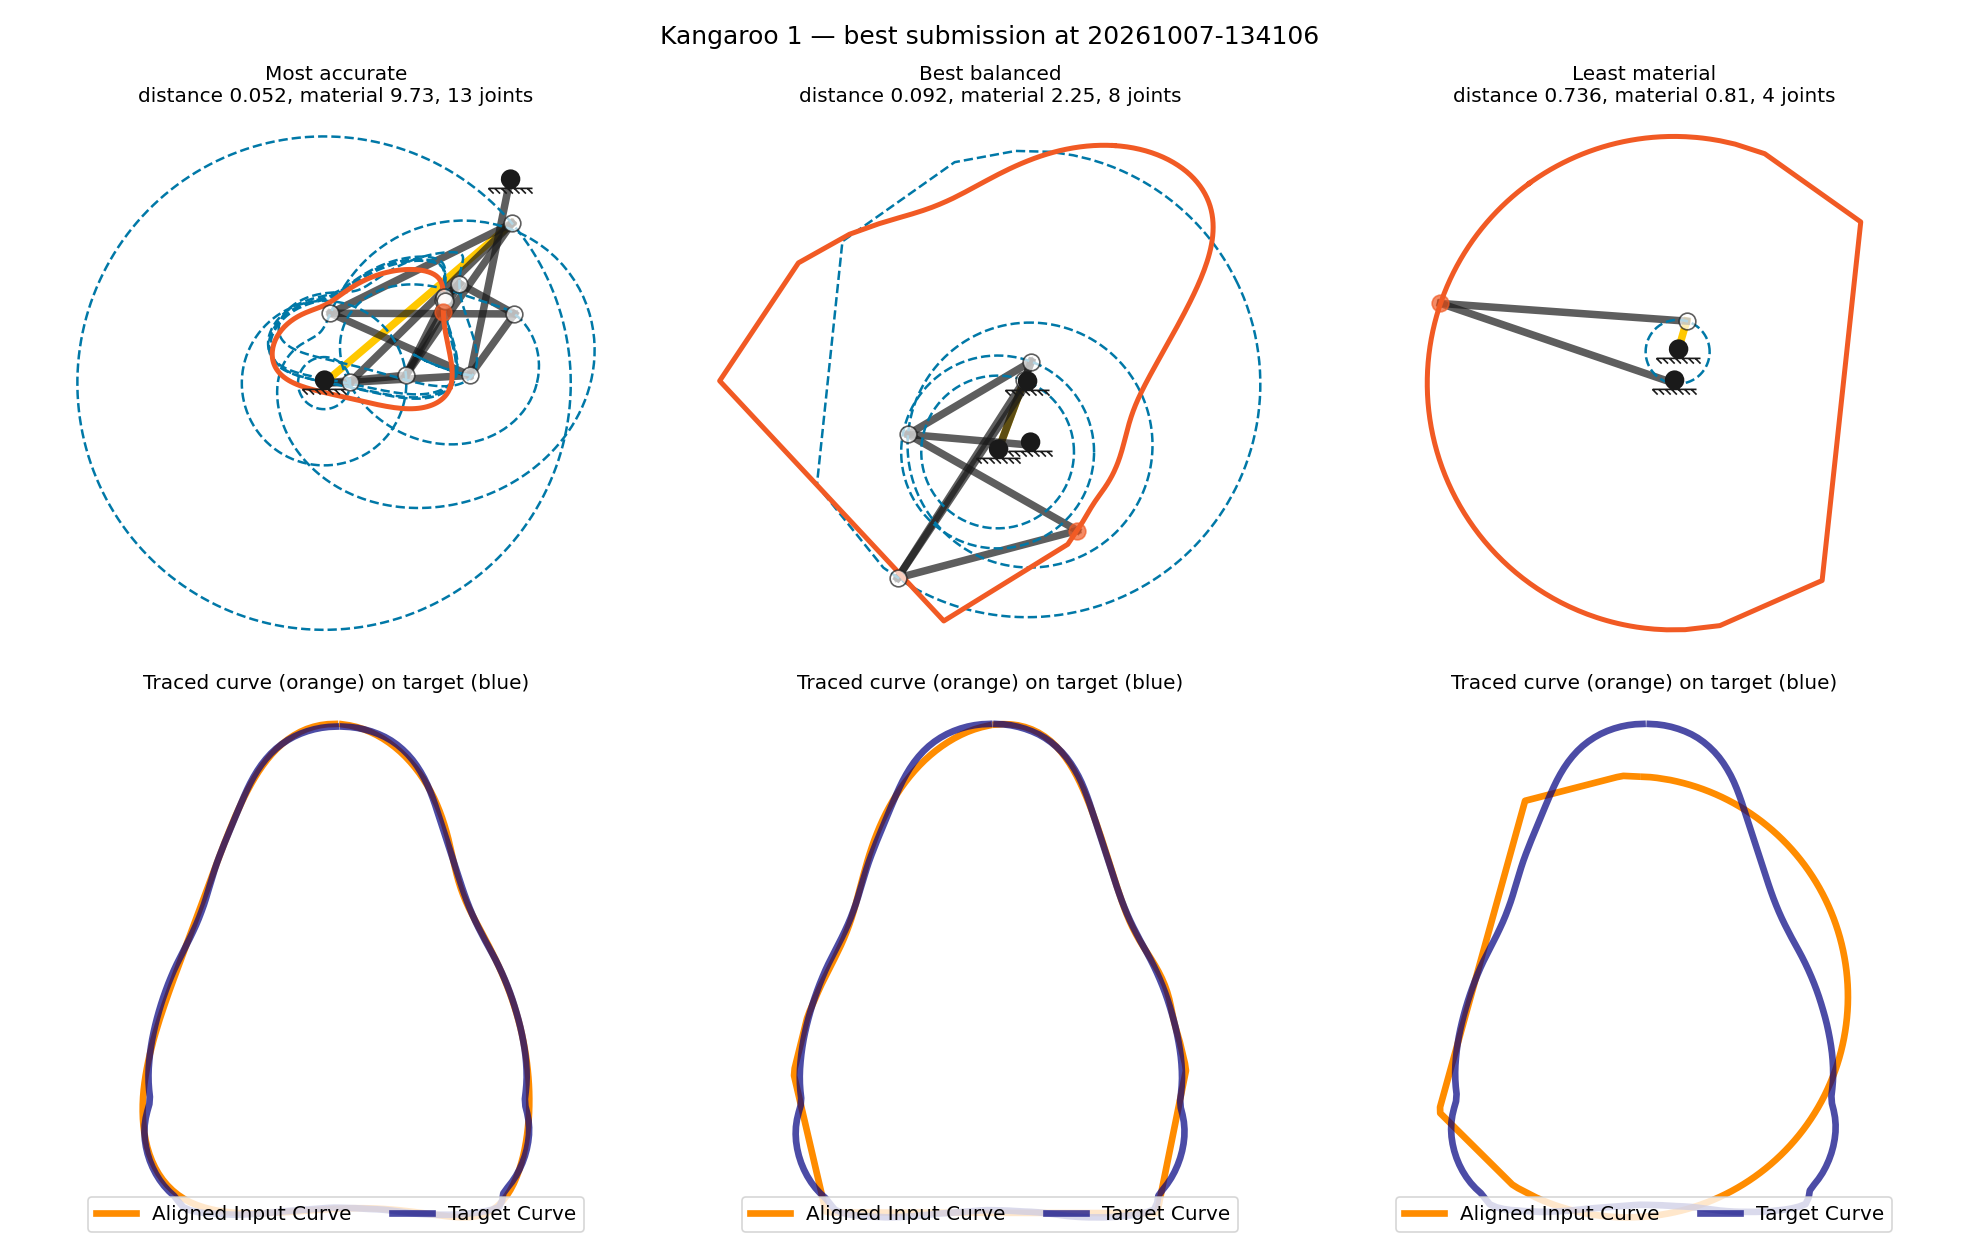
\includegraphics[width=0.92\linewidth]{best_1.png}
\caption{Kangaroo 1: mechanisms (top) and traced curves on the target (bottom).}
\label{fig:best1}
\end{figure}

\begin{figure}[H]
\centering
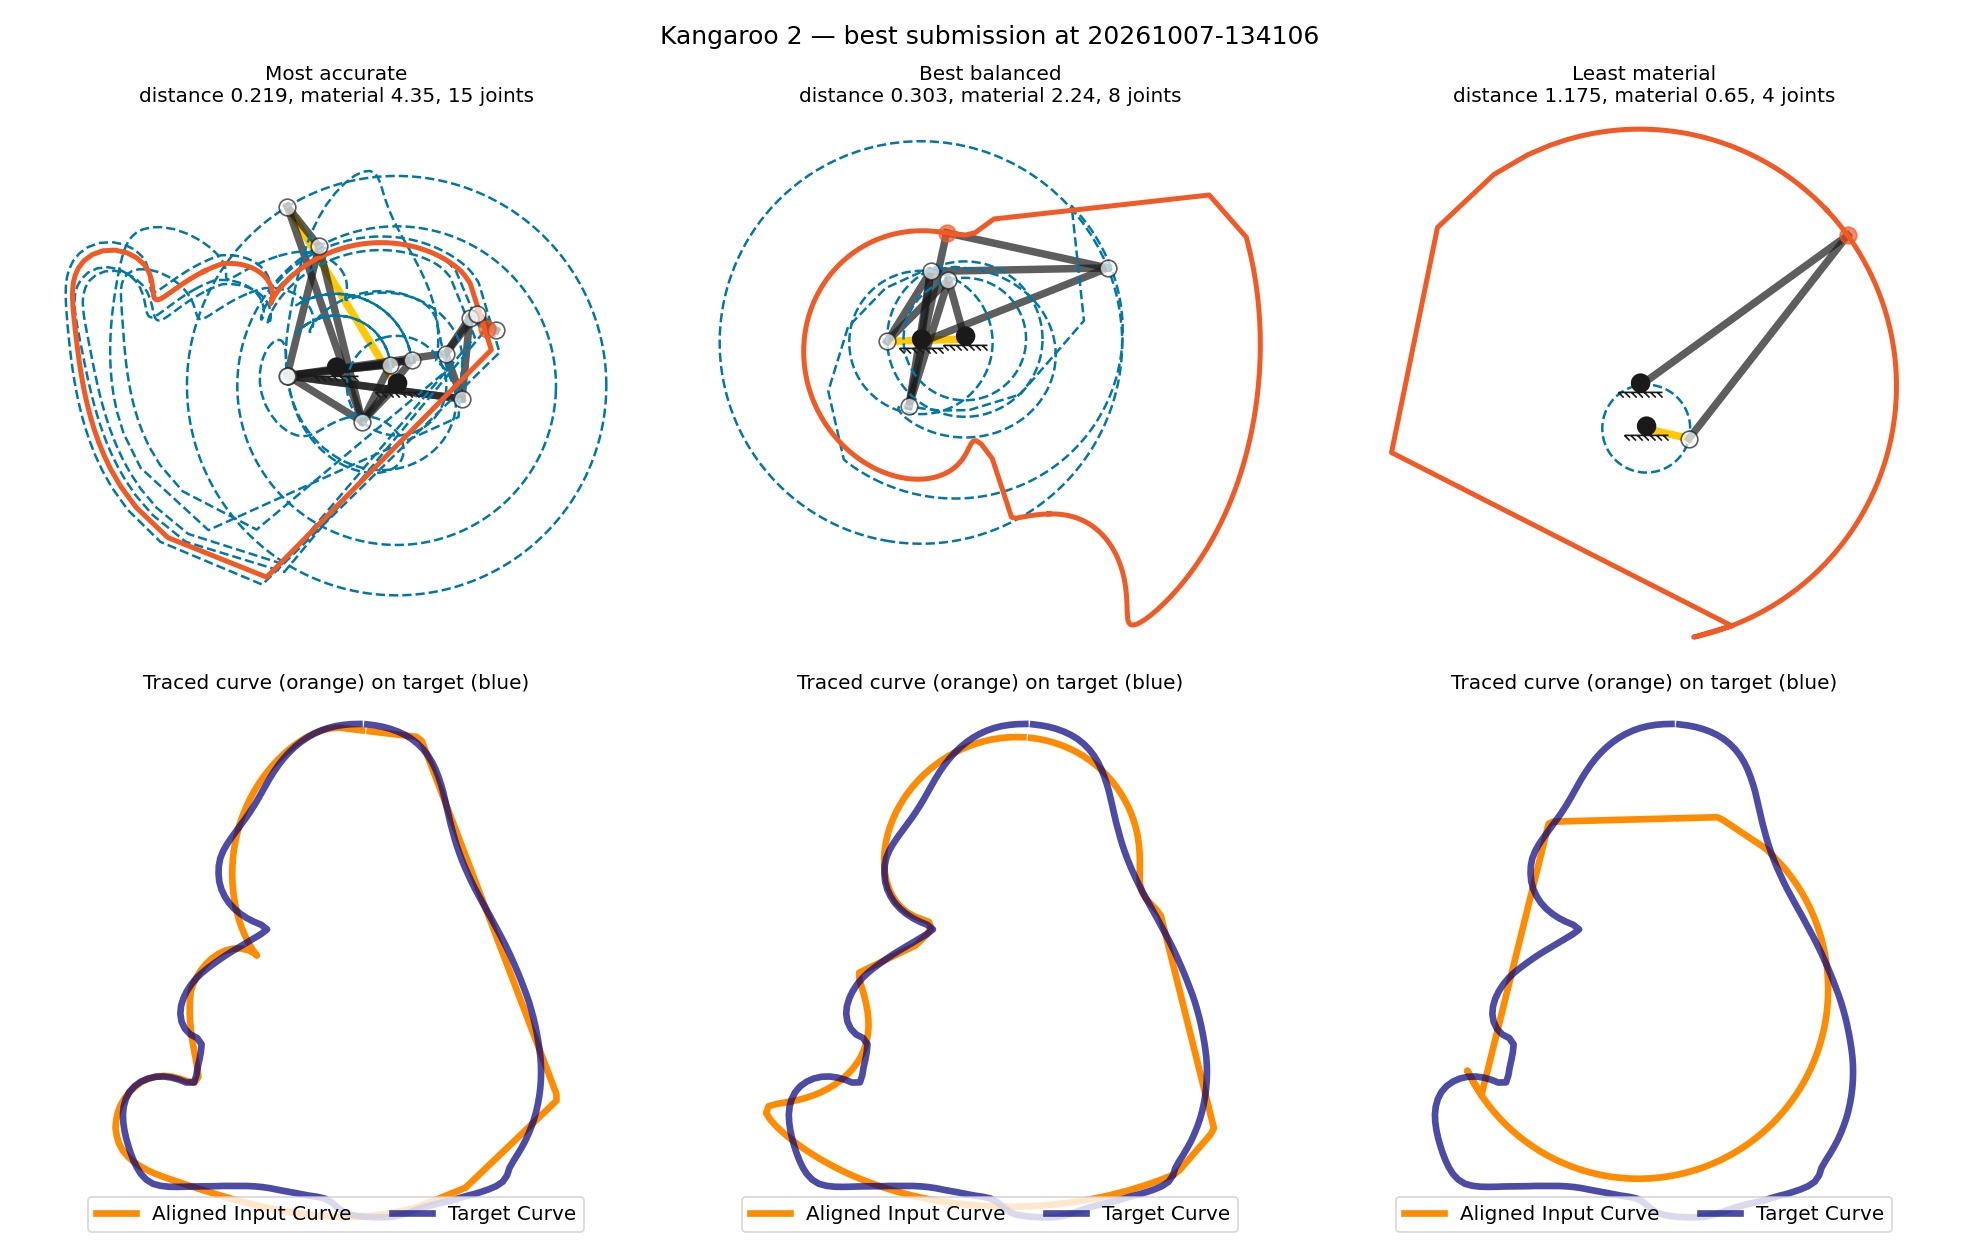
\includegraphics[width=0.92\linewidth]{best_2.png}
\caption{Kangaroo 2.}
\label{fig:best2}
\end{figure}

\begin{figure}[H]
\centering
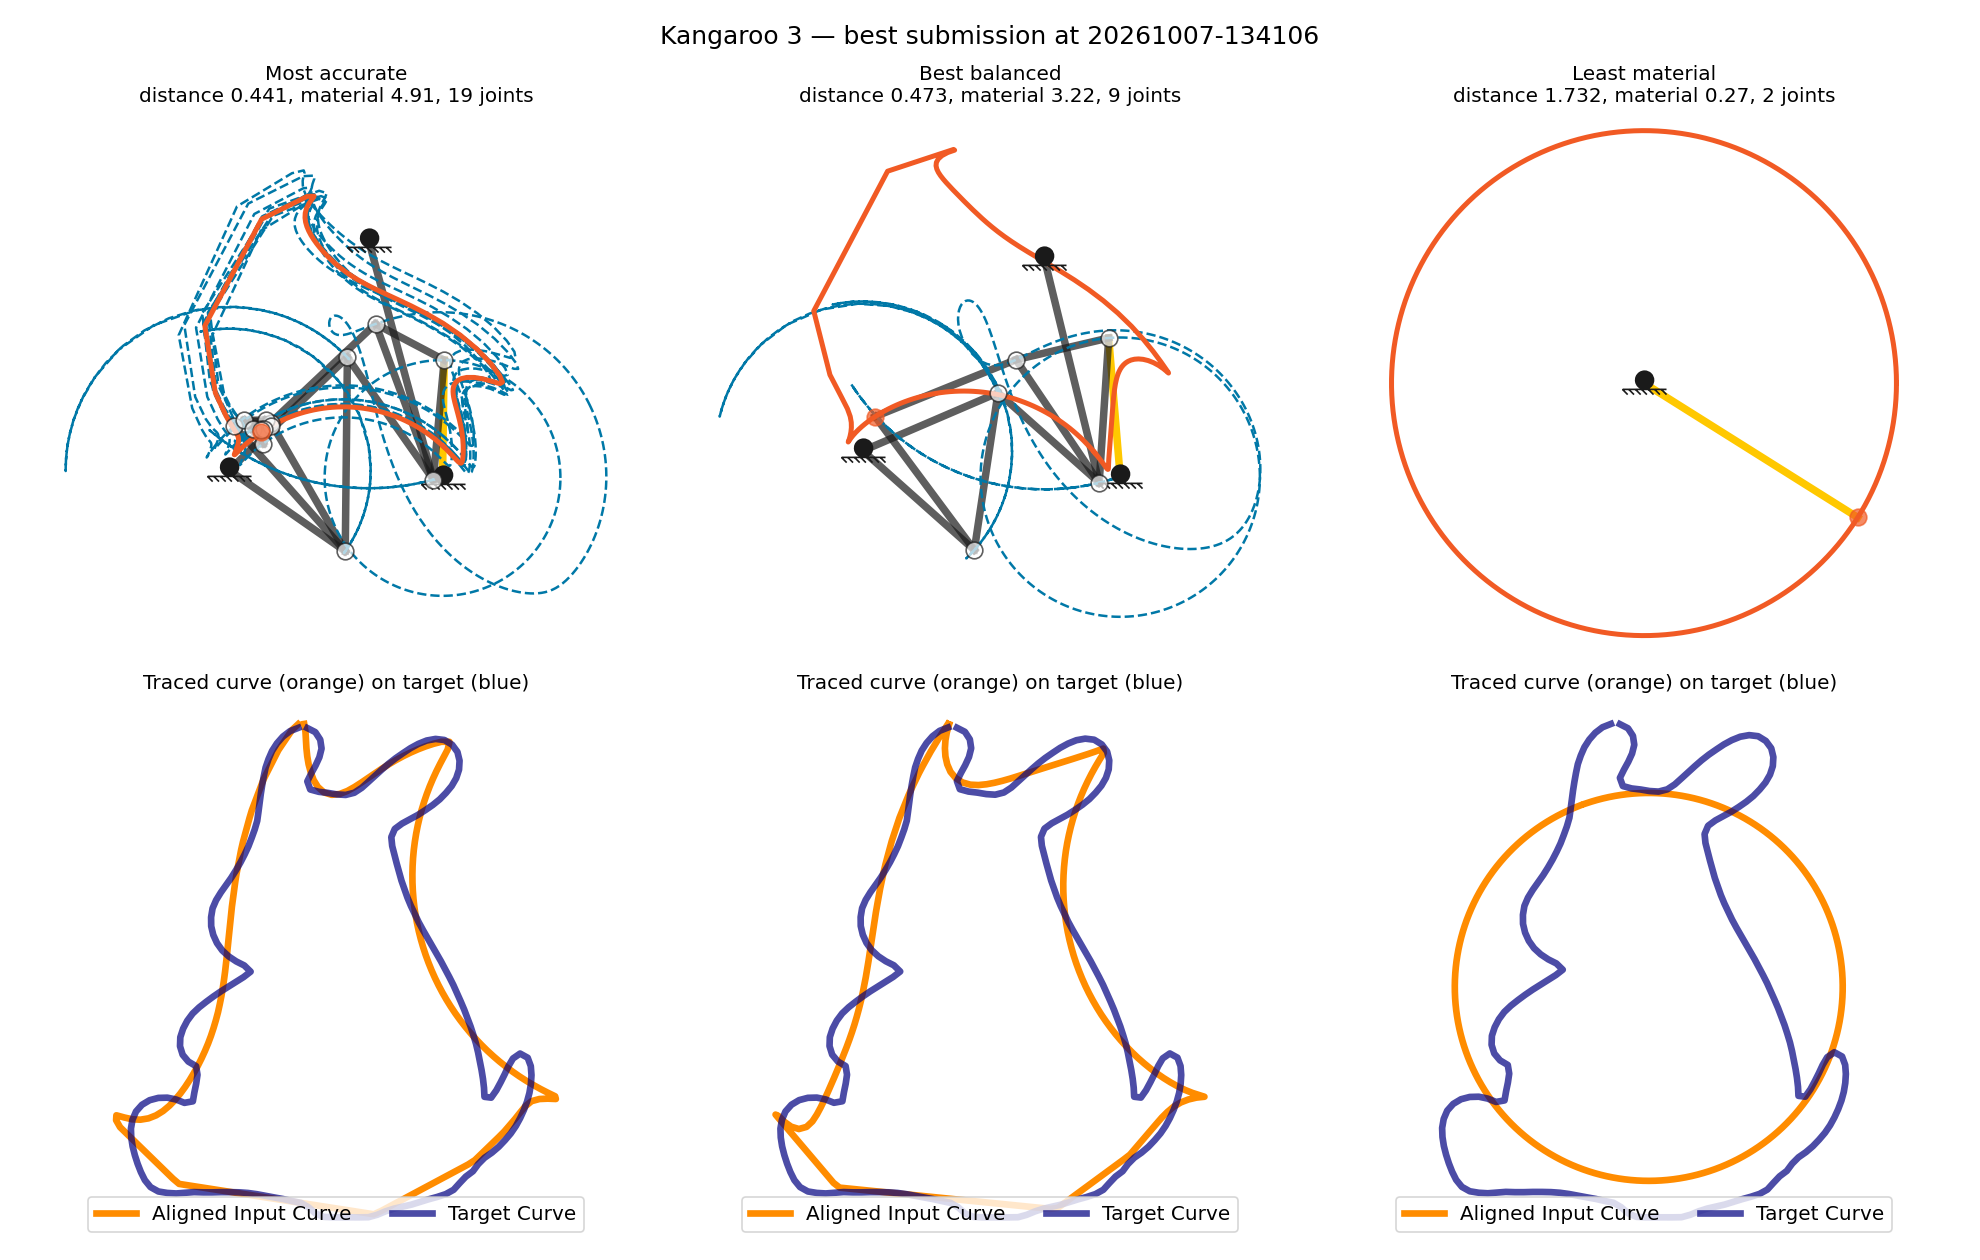
\includegraphics[width=0.92\linewidth]{best_3.png}
\caption{Kangaroo 3. The lightest design is a bare crank tracing a circle.}
\label{fig:best3}
\end{figure}

\section{Discussion}

\paragraph{Where the score came from.} Random screening alone reached 2.78 of
the final 3.69, and the first refinement added 0.65 more. Everything after
that added 0.26 in total. Of the later stages, the wide refinement added the
most (0.17), and it did so by making designs cheaper, not more accurate.

\paragraph{Accuracy against material.} For Kangaroo~1 the most accurate and
best-balanced designs are close in distance but far apart in material: the last
0.04 of distance costs more than four times the links. Kangaroo~2 shows the
same pattern more mildly. Kangaroo~3 is different: its most accurate and
best-balanced designs are close in both, and its front stops near a distance of
0.44 however much material is allowed. The material limit is not binding
there: the most accurate design uses 4.91 of the 20 allowed. It does use 19 of
the 20 joints allowed, but the ten joints it has beyond the best-balanced
design lower the distance only from 0.473 to 0.441, so we see no sign that a
higher joint limit alone would capture the missing detail. What is missing is
a link layout that traces the tail, and our search did not find one.

\paragraph{The bare crank.} The lightest Kangaroo~3 design is a two-joint
crank whose circle is just inside the distance limit. The course scorer accepts
it, but the submission page states 4 to 20 joints per mechanism, so it may not
be counted. It is worth 0.005 of Kangaroo~3's hypervolume.

\paragraph{What we would try next.} Since joint positions are exhausted, the
next step would be a structural search aimed at the tail: growth moves scored
by the error in the 55 to 65\% stretch of the perimeter instead of the total
distance, or a screen for sub-mechanisms that trace a narrow spike, attached to
the current best body.

\section{Compute and reproducibility}

Everything ran as CPU-only Slurm jobs on MIT ORCD Engaging, mostly on the
preemptable partition, where a job can be killed without warning. Every script
therefore checkpoints about once a minute and resumes exactly where it stopped.
Each stage merges its designs with the current best submission per problem,
re-scores with the course scorer, and keeps the result only if it is higher.
The file \texttt{CODE.md} in the code package describes each script and gives
the commands that reproduce the pipeline.

\end{document}
